\documentclass{beamer}
\usepackage{subfig}
\usepackage{amsmath}
\usepackage{bm}

\DeclareMathOperator*{\argmax}{arg\,max}
\DeclareMathOperator*{\argmin}{arg\,min}

\setbeamertemplate{footline}[frame number]
\title{Logistic Regression}
\author{Prof. Alessandro Lucantonio}
\institute{Aarhus University}
\date{}

\setbeamertemplate{navigation symbols}{}


\begin{document}
	\frame{\titlepage}
	
	\begin{frame}
		\frametitle{Binary classification}
		Recall: 
		\begin{itemize}
			\item Classification $\rightarrow$ discrete target.
			\item Binary classification: $\{0,1\}$ target (Ex.: spam/not spam).
		\end{itemize}
		
		\vspace{5mm}
		\textit{Idea}: consider a hypothesis (threshold) such that
		\begin{equation*}
			0 \leq h_{\bm{w}} \leq 1
		\end{equation*}
		and
		\begin{itemize}
			\item if $h_{\bm{w}}(\bm{x}) \geq 0.5$, predict $1$;
			\item if $h_{\bm{w}}(\bm{x}) < 0.5$, predict $0$.
		\end{itemize}
	\end{frame}

	\begin{frame}
		\frametitle{Logistic Regression}
		In particular, take $h_{\bm{w}}(\bm{x}) = \sigma(\bm{w}^T\bm{x})$, where
		\begin{equation*}
			\sigma(t) = \frac{1}{1+e^{-t}}
		\end{equation*}
		is the \textbf{sigmoid function}.
		$h_{\bm{w}}$ gives us the \textbf{probability} that the output is 1.
		\begin{figure}
			\centering
			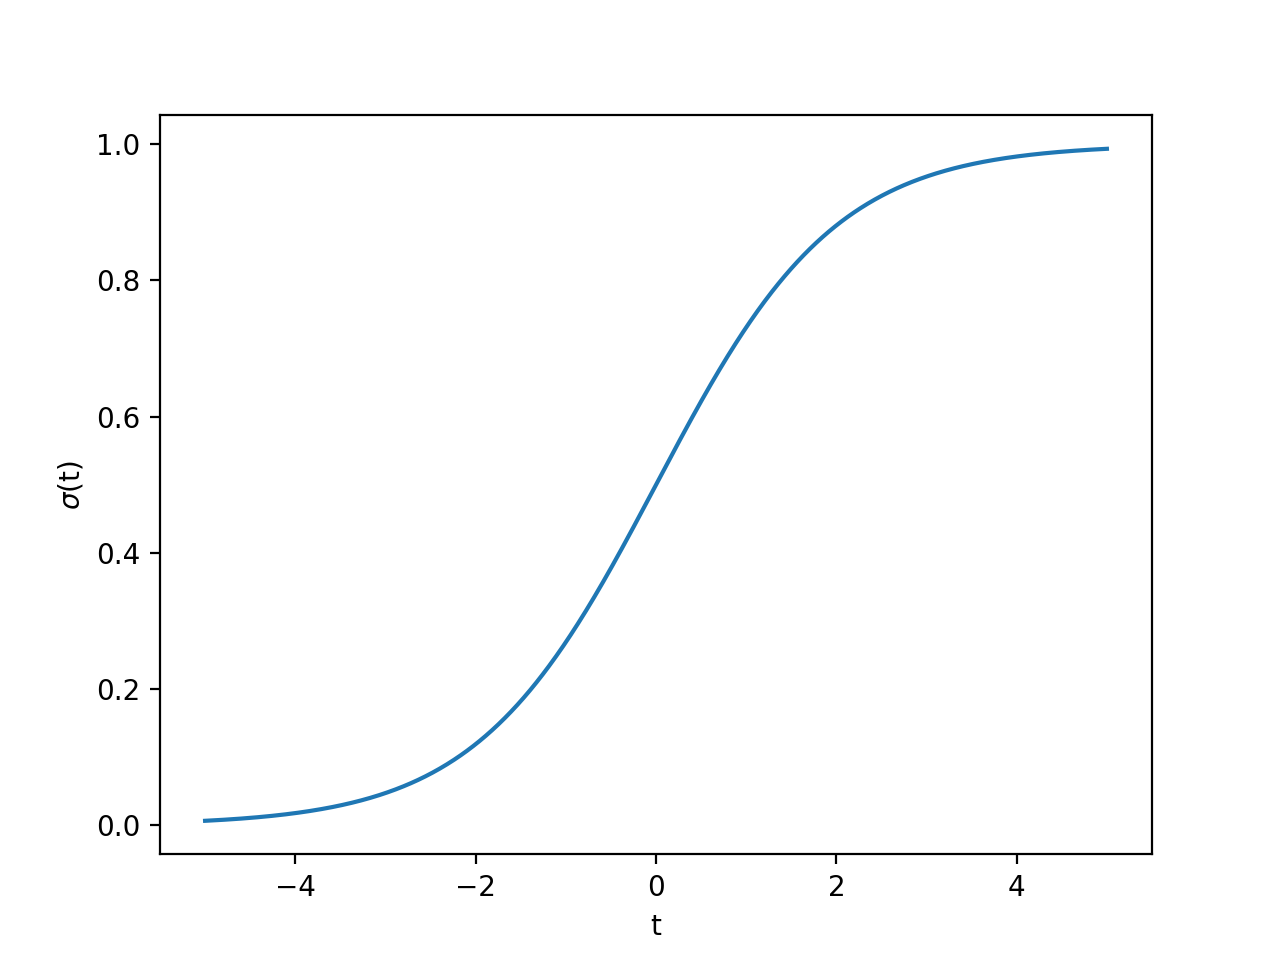
\includegraphics[scale=0.42]{images/sigmoid}
			\caption{Sigmoid function.}
		\end{figure}
		
	\end{frame}

	\begin{frame}
		\frametitle{Linear decision boundary}
		Hypothesis: $h_{\bm{w}}(x_1, x_2) = \sigma(w_0 + w_1 x_1 + w_2 x_2)$
		
		\vspace{2mm}
		
		$h_{\bm{w}}(x_1, x_2) \geq 0.5$ when $w_0 + w_1 x_1 + w_2 x_2 \geq 0 \implies y = 1$
		$h_{\bm{w}}(x_1, x_2) < 0.5$ when $w_0 + w_1 x_1 + w_2 x_2 < 0 \implies y = 0$
		
		\vspace{1mm}
		
		The decision boundary is \textbf{not unique} in the \textit{linearly separable case} unless additional constraints, like \textit{regularization}, are applied.
		
		\begin{figure}
			\centering
			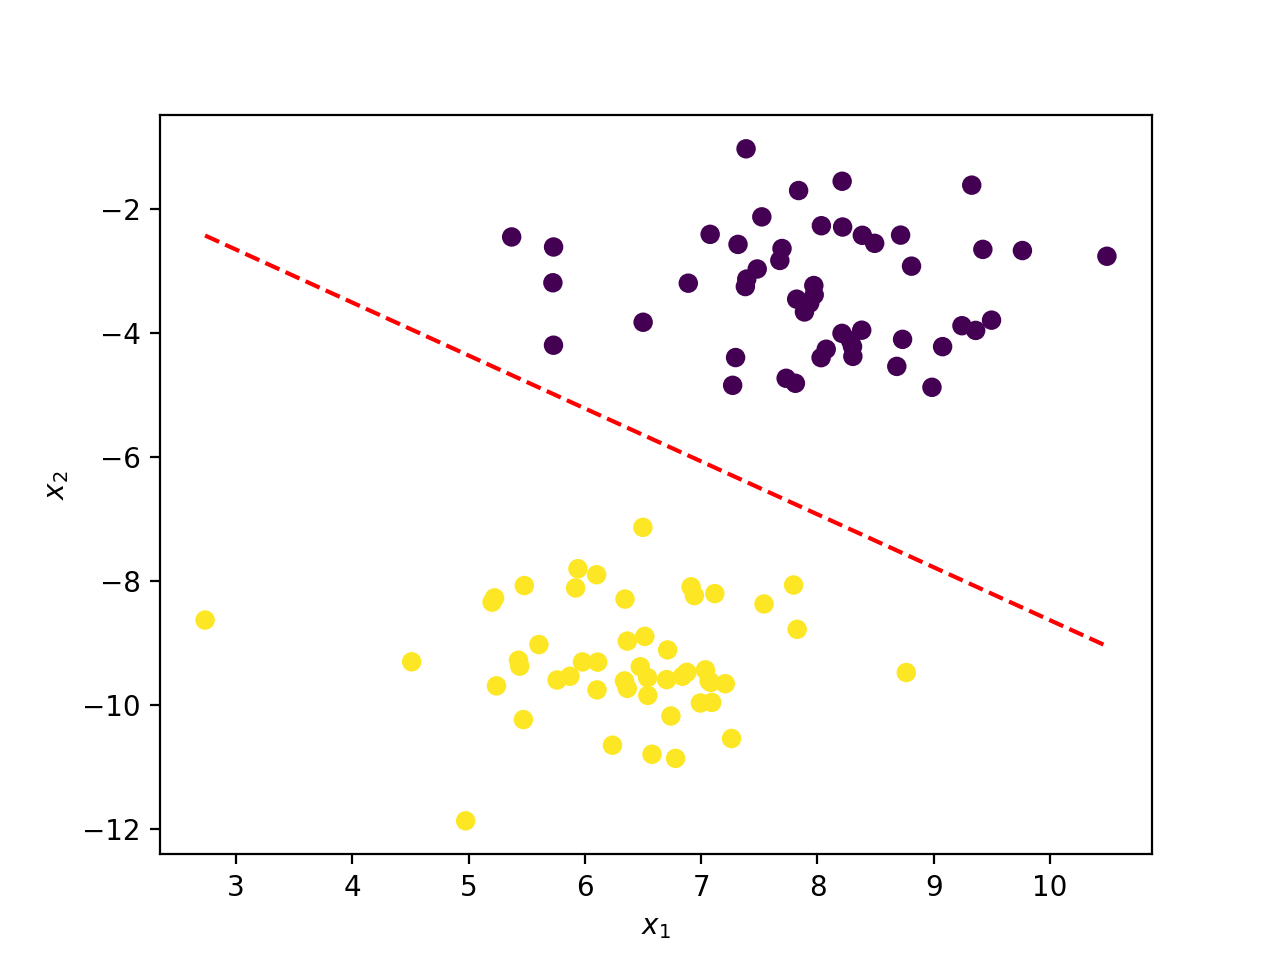
\includegraphics[scale=0.38]{images/linear_decision_boundary}
			\caption{An example of linear decision boundary for the linearly separable case.}
		\end{figure}
	\end{frame}

	\begin{frame}
		\frametitle{Non-linear decision boundary}
		Hypothesis: $h_{\bm{w}}(x_1, x_2) = \sigma(w_0 + w_1 x_1 + w_2 x_2 + w_3 x_1^2 + w_4 x_2^2)$
		\begin{figure}
			\centering
			
\includegraphics[scale=0.8]{images/non-linear-decision-boundary}
			\caption{An example of non-linear decision boundary.}
		\end{figure}
	\end{frame}

	\begin{frame}
		\frametitle{Cost function}
		
		First attempt: MSE
		\begin{equation*}
			E(\bm{w}) = \frac{1}{N} \sum_{i= 0}^{N} (\sigma(\bm{w}^T\tilde{\bm{x}}^{(i)}) - y^{(i)})^2
		\end{equation*}
		
		Problem: $\sigma$ is \textsl{non-convex}, hence MSE is \textsl{non-convex} (possibly many local minima).
		
		\vspace{5mm}
		
		Main idea: consider the a loss term that behaves as
		\begin{itemize}
			\item $-\log h_{\bm{w}}(\tilde{\bm{x}}^{(i)})$ if $y=1$, 
			\item $-\log (1-h_{\bm{w}}(\tilde{\bm{x}}^{(i)}))$ if $y=0$
		\end{itemize}
		
		Notice that:
		\begin{itemize}
			\item if $y=1$ and $h_{\bm{w}}(\tilde{\bm{x}}^{(i)}) \rightarrow 1$, $-\log h_{\bm{w}}(\tilde{\bm{x}}^{(i)}) \rightarrow 0$;
			\item if $y=1$ and $h_{\bm{w}}(\tilde{\bm{x}}^{(i)}) \rightarrow 0$, $-\log h_{\bm{w}}(\tilde{\bm{x}}^{(i)}) \rightarrow \infty$;
			\item if $y=0$ and $h_{\bm{w}}(\tilde{\bm{x}}^{(i)}) \rightarrow 1$, $-\log (1-h_{\bm{w}}(\tilde{\bm{x}}^{(i)})) \rightarrow \infty$;
			\item if $y=0$ and $h_{\bm{w}}(\tilde{\bm{x}}^{(i)}) \rightarrow 0$, $-\log (1-h_{\bm{w}}(\tilde{\bm{x}}^{(i)})) \rightarrow 0$;
		\end{itemize}

	\end{frame}
	
	\begin{frame}
		\frametitle{Cross-entropy}
		Combine the log loss terms: \textbf{Binary cross-entropy}
		\begin{equation*}
			E(\bm{w}) := - \frac{1}{N} \sum_{i=1}^{N} y^{(i)}\log(h_{\bm{w}}(\tilde{\bm{x}}^{(i)})) + (1-y^{(i)})\log(1-h_{\bm{w}}(\tilde{\bm{x}}^{(i)}))
		\end{equation*}
		This cost function is \textit{convex} (sum of convex terms) with respect to the weights.
		
		\vspace{5mm}
		Vectorized version:
		\begin{equation*}
			E(\bm{w}) = - \frac{1}{N} \left(\bm{y}^T\log (h_{\bm{w}}(\mathsf{X})) + (1-\bm{y}^T)\log(1-h_{\bm{w}}(\mathsf{X}))\right)
		\end{equation*}
		with $h_{\bm{w}}(\mathsf{X}) = \sigma(\mathsf{X}\bm{w})$.
	\end{frame}

	\begin{frame}
	\frametitle{Conditional Log-Likelihood and Binary Cross-Entropy}
	In a \textit{binary classification} problem, the model provides a joint probability of the form
	$$P(y^{(i)} | x^{(i)}; \bm{\theta}) = (\hat{y}^{(i)})^{y^{(i)}} (1-\hat{y}^{(i)})^{(1-{y}^{(i)})}$$
	The log-likelihood is:
	$$\sum_{i=1}^{N}\log P(y^{(i)} | x^{(i)}; \bm{\theta}) = \sum_{i=1}^{N}y^{(i)}\log(\hat{y}^{(i)}) + (1-{y}^{(i)})\log(1-\hat{y}^{(i)})$$
	which is the \textbf{binary cross-entropy loss}.
\end{frame}

	\begin{frame}
		\frametitle{Convexity}
		Any local minimum of a convex function is also a global minimum. 
		Instead, a non-convex function has potentially many local minima and \textit{saddle points} (vanishing gradient but neither minimum nor maximum).
		
		\begin{figure}
			\centering
			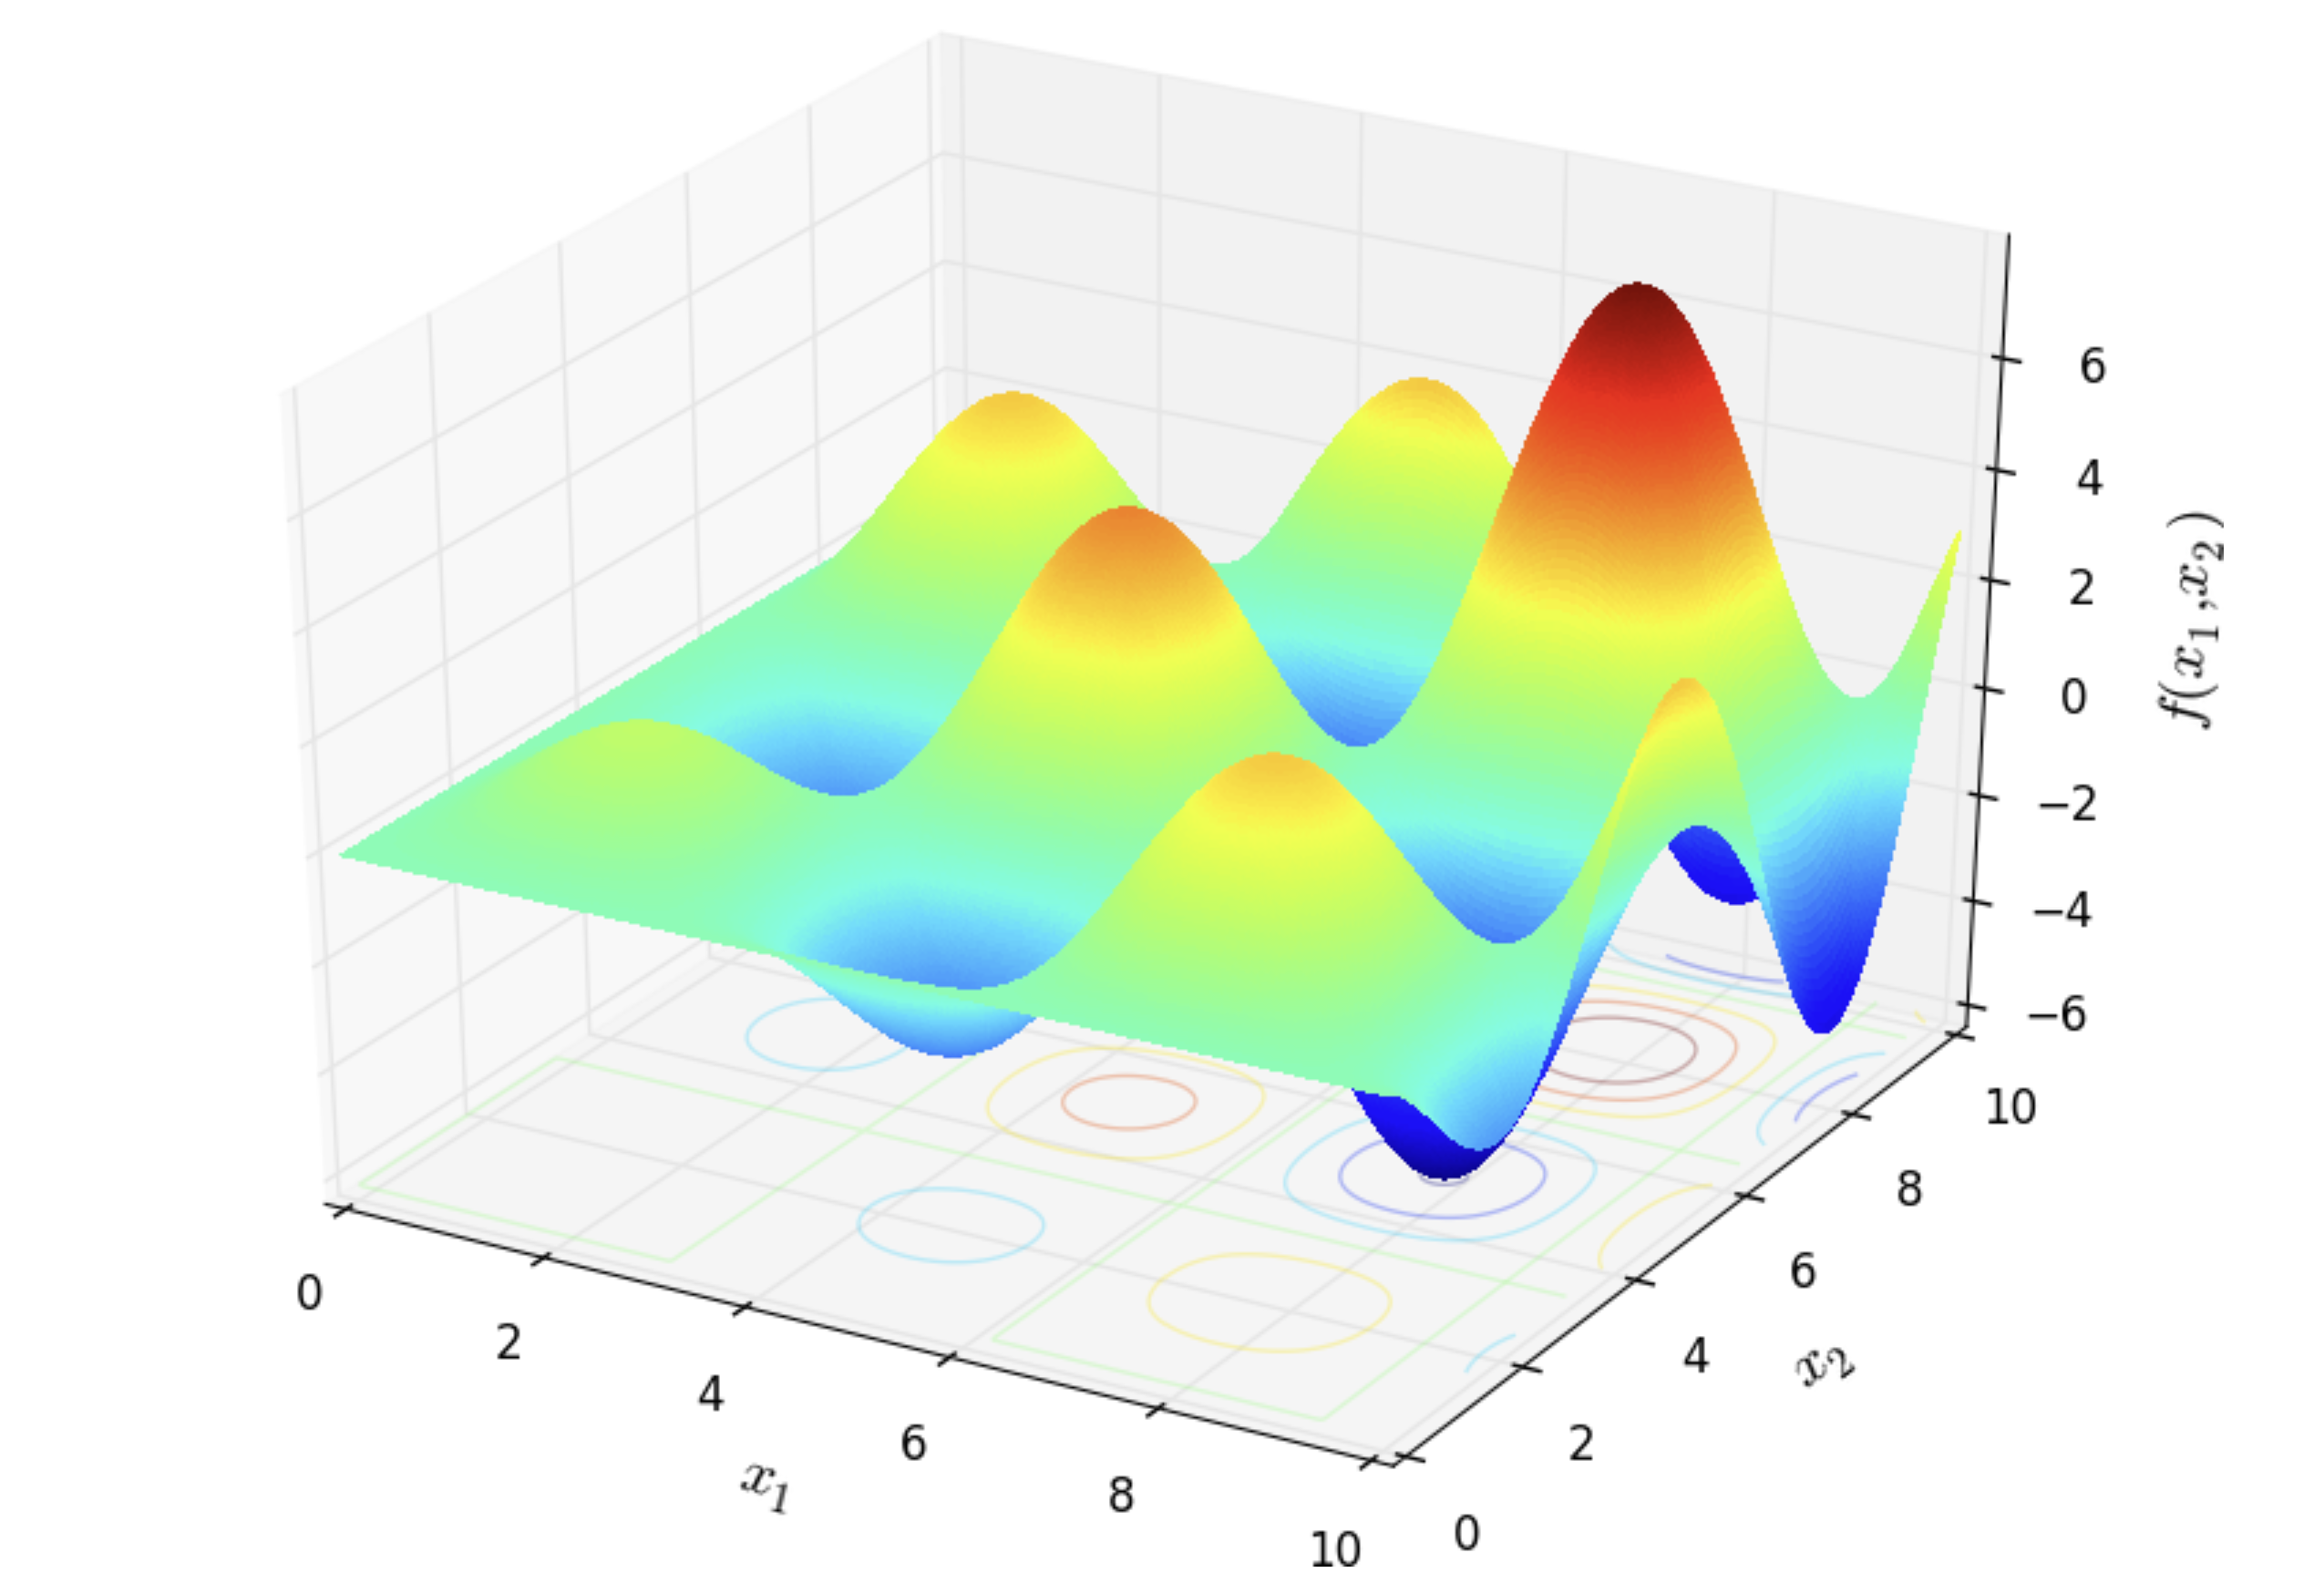
\includegraphics[scale=0.25]{images/non_convex}
			\caption{An example of a non-convex function.}
		\end{figure}
		
		%Remember the main challenge/goal of ML: \textbf{generalization}.  A global minimum of the cost function corresponds to the best fit of the training set: this may lead to \textbf{overfitting}.
	\end{frame}

	\begin{frame}
		\frametitle{Is a local minimum always bad?}
		
		Answer: NO; remember the main challenge/goal of ML: \textbf{generalization}.
		
		\vspace{2mm}
		
		\begin{itemize}
			\item A global minimum of the cost function corresponds to the best fit of the training set: this may lead to \textbf{overfitting}.
			\item Having a convex cost function is convenient, but finding a local minimum is probably even better than a global minimum. 
			\item Saddle points may be bottlenecks for gradient-based optimization, but there are techniques to avoid them (momentum, learning rate schedules, \dots) in modern optimization algorithms.
		\end{itemize}
%		
%		%Worst case scenario: find a saddle point.
	\end{frame}

	\begin{frame}
		\frametitle{Gradient descent - Derivative of the sigmoid}
		For gradient descent-based optimization, we need to compute the gradient of the cross-entropy with respect to the weights.
		
		\vspace{5mm}
		
		Recall: $\sigma(t) := \frac{1}{1+e^{-t}}$.
		
		\begin{align*}
			\frac{\textrm{d}}{\textrm{d}t} \sigma(t) &= \frac{e^{-t}}{(1 + e^{-t})^2}\\
			&= \left(\frac{1}{1 + e^{-t}}\right)\left(\frac{e^{-t}}{1 + e^{-t}}\right)\\
			&= \sigma(t)\left(1 - \frac{1}{1 + e^{-t}}\right)\\
			&= \sigma(t)(1 - \sigma(t)).
		\end{align*}
		
	\end{frame}

	\begin{frame}
		\frametitle{Gradient of the cross-entropy /1}
	
		(assuming sum on repeated indices)
		\begin{align*}
			N\frac{\partial}{\partial \bm{w}_j} E(\bm{w}) &= - \left[\frac{y^{(i)} \frac{\partial}{\partial \bm{w}_j}h_{\bm{w}}(\tilde{\bm{x}}^{(i)})}{h_{\bm{w}}(\tilde{\bm{x}}^{(i)})} - \frac{(1-y^{(i)}) \frac{\partial}{\partial \bm{w}_j}(1 -h_{\bm{w}}(\tilde{\bm{x}}^{(i)}))}{1-h_{\bm{w}}(\tilde{\bm{x}}^{(i)})}\right]\\
		\end{align*}
		with
		\begin{align*}
			\frac{\partial}{\partial \bm{w}_j} h_{\bm{w}}(\tilde{\bm{x}}^{(i)}) &= \sigma'(\bm{w}^T \tilde{\bm{x}}^{(i)}) \tilde{\bm{x}}^{(i)}_j = \sigma(\bm{w}^T\tilde{\bm{x}}^{(i)})(1 - \sigma(\bm{w}^T \tilde{\bm{x}}^{(i)}))\tilde{\bm{x}}^{(i)}_j\\
			&= h_{\bm{w}}(\tilde{\bm{x}}^{(i)})(1 - h_{\bm{w}}(\tilde{\bm{x}}^{(i)}))\tilde{\bm{x}}^{(i)}_j 
		\end{align*}
	
	\mbox{}\hfill $\rightarrow$
	
	\end{frame}

	\begin{frame}
		\frametitle{Gradient of the cross-entropy /2}
		\begin{align*}
			N\frac{\partial}{\partial \bm{w}_j} E(\bm{w})&= -[y^{(i)}(1 - h_{\bm{w}}(\tilde{\bm{x}}^{(i)}))\tilde{\bm{x}}^{(i)}_j - (1-y^{(i)})h_{\bm{w}}(\tilde{\bm{x}}^{(i)})\tilde{\bm{x}}^{(i)}_j]\\
			& = [h_{\bm{w}}(\tilde{\bm{x}}^{(i)})- y^{(i)}]\tilde{\bm{x}}^{(i)}_j.
		\end{align*}
	Final result:
		\begin{align*}
			\frac{\partial}{\partial \bm{w}_j} E(\bm{w}) = \frac{1}{N} \sum_{i=0}^{N} [h_{\bm{w}}(\tilde{\bm{x}}^{(i)})- y^{(i)}]\tilde{\bm{x}}^{(i)}_j.
		\end{align*}
	
	Vectorized version:
	\begin{align*}
		\nabla E(\bm{w}) = \frac{1}{N} \mathsf{X}^T(\sigma(\mathsf{X}\bm{w}) - \bm{y}).
	\end{align*}
	
	\end{frame}

	\begin{frame}
		\frametitle{Multi-class classification}
		
		Targets: $y \in \{0, \dots, k\}$.
		
		\vspace{5mm}
		
		Idea: solve $k+1$ binary classification problems. Given a data sample $\bm{x}^{(i)}$:
		\begin{itemize}
			\item For each $0\leq j \leq k$, compute the probability $h^{(j)}_{\bm{w}}(\tilde{\bm{x}}^{(i)})$ that $\tilde{\bm{x}}^{(i)}$ belongs to the class $j$.
			\item The prediction will be the class that corresponds to the maximum probability, \textit{i.e.} 
			$$\argmax_j h^{(j)}_{\bm{w}}(\tilde{\bm{x}}^{(i)})\ .$$
		\end{itemize}
		
		
	\end{frame}
\end{document}